%%+++++++++++++++++++++++++++++++++++++%%
%%         Final Version  6/14/95      %%
%%+++++++++++++++++++++++++++++++++++++%%
\documentclass[12pt]{article}
\textheight = 8.6in
\textwidth = 6.2in
\topmargin = -.5in
\oddsidemargin = 0.08in
\evensidemargin = 0.08in
%\usepackage{fancyhdr}
%\pagestyle{fancy}
%\rfoot{\thepage}
\setlength{\jot}{10.0 pt}
\setlength{\parskip}{2.0ex}
\setlength{\footskip}{65pt}

\usepackage{graphicx}
\usepackage{subfigure}
\usepackage{placeins}
\usepackage{afterpage}
\usepackage{amsmath}
\usepackage{empheq}
\usepackage[most]{tcolorbox}
\newtcbox{\mymath}[1][]{%
    nobeforeafter, math upper, tcbox raise base,
    enhanced, colframe=white!20!black ,
    colback=blue!30!red!30!white, boxrule=1pt,
    #1}
\usepackage{xcolor}
\definecolor{myblue}{RGB}{0, 0, 180}   %Numbers are integers from 0 to 255, smaller is closer to black
\definecolor{grey}{RGB}{200, 200, 200}   %Numbers are integers from 0 to 255, smaller is closer to black
\definecolor{mygreen}{RGB}{0, 100, 0}   %Numbers are integers from 0 to 255, smaller is closer to black
\definecolor{myred}{RGB}{120, 0, 0}   %Numbers are integers from 0 to 255, smaller is closer to black

\begin{document}

\begin{flushright} {\color{blue} Chapter 3, Lecture 4} \end{flushright}
\begin{flushleft}

\subsubsection*{\color{myblue} \bf Separation of Variables: Laplace's equation in 2D spherical coordinates}

Separation of variables is a technique for finding a solution to a partial differential equation (such as Laplace's equation).  In this method, a solution is postulated that is a product of functions, each of these functions in only one of the independent variables.  This product solution is substituted into the partial differential equation, in hopes of going to two or three ordinary differential equations, each one in terms of only one of the independent variables.  If this can be done, then each ordinary differential equation is considered separately to find a functional form of the solution for this independent variable.  Laplace's equation is solvable using the separation of variables technique.

Consider the Laplace equation in spherical coordinates when the voltage has no azimuthal ($\phi$) dependence, we have $V(r,\theta)$ and so no $\phi$ derivative in Laplace's equation,

\begin{equation*}
\begin{aligned}
& \nabla^{2}V(r,\theta) = 0 \\[6pt]
& \frac{1}{r^{2}}\frac{\partial}{\partial r}\left( r^{2} \frac{\partial V(r,\theta)}{\partial r} \right) + \frac{1}{r^{2}\sin{(\theta)}} \frac{\partial}{\partial \theta} \left(\sin{(\theta)} \frac{\partial V(r,\theta)}{\partial \theta} \right) = 0
\end{aligned}
\end{equation*}

Write $V(r,\theta)$ as a product of functions, each dependent on only one of the independent variables, $V(r,\theta)=\mathcal{R}(r)\Theta(\theta)$.  Substituting this into Laplace's equation,

\begin{equation}
\frac{\Theta(\theta)}{r^{2}}\frac{\partial}{\partial r}\left( r^{2} \frac{\partial \mathcal{R}(r)}{\partial r} \right) + \frac{\mathcal{R}(r)}{r^{2}\sin{(\theta)}} \frac{\partial}{\partial \theta} \left(\sin{(\theta)} \frac{\partial \Theta(\theta)}{\partial \theta} \right) = 0 
\label{eq:productthere}
\end{equation}

Now multiply both sides of Eq.~\ref{eq:productthere} by $\frac{r^{2}}{\mathcal{R}(r)\Theta(\theta)}$:

\begin{equation}
\frac{1}{\mathcal{R}(r)}\frac{\partial}{\partial r}\left( r^{2} \frac{\partial \mathcal{R}(r)}{\partial r} \right) + \frac{1}{\Theta(\theta)\sin{(\theta)}} \frac{\partial}{\partial \theta} \left(\sin{(\theta)} \frac{\partial \Theta(\theta)}{\partial \theta} \right) = 0
\label{eq:independentterms}
\end{equation}

The first term of Eq.~\ref{eq:independentterms} has only $r$-dependence, while the second term of Eq.~\ref{eq:independentterms} has only $\theta$-dependence.  Therefor each term must be equal to a constant.   This time, for later convenience, we will set this constant equal to $\pm l(l+1)$, where $l$ is an integer.  Then we have the two following equations (one for each term),

\begin{align}
&  \frac{1}{\mathcal{R}(r)}\: \frac{d}{dr}\left( r^{2} \frac{d\mathcal{R}(r)}{dr} \right) = l(l+1) \label{eq:req} \\[6pt]
& \frac{1}{\Theta(\theta)\sin{(\theta)}} \: \frac{d}{d\theta} \left(\sin{(\theta)} \frac{d\Theta(\theta)}{d\theta} \right) = -l(l+1) \label{eq:thetaeq}
\end{align}

Notice that equations \ref{eq:req} and \ref{eq:thetaeq} are now ordinary differential equations, the solutions of which are known.  You can check the following solution to Eq.~\ref{eq:req} by direct substitution:

\[
\mathcal{R}(r) = Ar^{l}+\frac{B}{r^{l+1}}
\]

Eq.~\ref{eq:thetaeq} is Legendre's differential equation (often written with $x$ instead of $\cos{(\theta)}$) which has a known solution, the Legendre polynomial of order $l$.  That is,

\[
\Theta(\theta) = P_{l}(\cos{(\theta)})
\]

Our choice of constant $l$ was arbitrary, so sum $V(r,\theta) = \mathcal{R}(r)\Theta(\theta)$ over all possible integer values of $l$ to have the general solution:

\tcbset{highlight math style={colframe=myblue,colback=white}}
\begin{empheq}[box=\tcbhighmath]{equation}
V(r,\theta) = \sum_{l=0}^{\infty} \left(  A_{l}r^{l} + B_{l}r^{-(l+1)} \right) P_{l}(\cos{(\theta)})
 \end{empheq}

An example for a spherical boundary problem follows.  It has some general pointers in addition to the solution for a specific situation.

 \vspace{.2in}
{\color{grey} \rule{\linewidth}{0.7mm} }\\
\vspace{-.2in}
{\textbf{\color{mygreen} Example problem: Spherical shell}}\\
\vspace{.1in}
It is not necessary to solve Laplace's equation from the beginning if the general solution appropriate to the geometry is already known.  For spherical geometry with no $\Phi$ dependence, the expansion for the potential is written:

\begin{equation*}
 V(r,\theta) = \sum_{l=0}^{\infty} \left(  A_{l}r^{l} + B_{l}r^{-(l+1)} \right) P_{l}(\cos{(\theta)})
\end{equation*}

Then we follow the general steps below:
\begin{enumerate} 
\item Write out the boundary conditions for the problem at hand. 
\item Apply the general (often zero voltage/charge in some limit) boundary conditions to simplify the general solution.
\item Apply the voltage/charge B.C. specific to the problem at hand, solving for the last undetermined coefficient using the properties of orthogonal functions.
\end{enumerate}

Before doing a specific problem, consider boundary value problems with a spherical shell as the boundary in general.  A spherical shell of radius $r=R$ splits space into two regions; a region where $r<R$, with a voltage function that we'll call $V_{\text{in}}(r,\theta)$, and a region where $r>R$, with a voltage function that we'll call $V_{\text{out}}(r,\theta)$.  For \textit{any} problem, the following B.C. holds:

\begin{equation}
V_{\text{in}}(R,\theta) = V_{\text{out}}(R,\theta)
\label{eq:inout}
\end{equation}

Or, stating that another way,

\[
\left. V_{\text{in}}(r,\theta) = V_{\text{out}}(r,\theta) \: \right|_{r=R}
\]

We'll get back to Eq.~\ref{eq:inout} soon.

For all of the spherical geometry problems in this course, 

\begin{equation}
V_{\text{in}}(r,\theta)   \hspace{.05in} \text{is finite as} \hspace{.1in} r\rightarrow 0 
\label{eq:bc1}
\end{equation}

Considering the limit given by Eq.~\ref{eq:bc1}:
\begin{align}
& V_{\text{in}}(r\rightarrow 0, \theta)=\lim\limits_{r \to 0} \: \sum_{l=0}^{\infty} \left(  A_{l}r^{l} + B_{l}r^{-(l+1)} \right) P_{l}(\cos{(\theta)})  \hspace{.1in} \text{is finite} \notag \\[2pt]
& \lim\limits_{r \to 0} \: A_{l}r^{l} =A_{0} \notag \\[2pt]
& \lim\limits_{r \to 0} \: B_{l}r^{-(l+1)} \rightarrow \infty \hspace{1in} \text{\color{myblue} This term blows up!} \notag 
\end{align}

Since the $B_{l}r^{-(l+1)}$ terms blow up as $r\rightarrow 0$, all the $B_{l}$ coefficients of $V_{\text{in}}$ must be zero.  That is,

\begin{equation}
 V_{\text{in}}(r,\theta) = \sum_{l=0}^{\infty} A_{l}r^{l} P_{l}(\cos{(\theta)})
\label{eq:vin}
\end{equation}

For most (but not all!) of the spherical boundary value problems in the course, 
\begin{equation}
V_{\text{out}}(r,\theta) = 0 \hspace{.1in} \text{as} \hspace{.1in} r\rightarrow \infty 
\label{eq:bc2}
\end{equation}

If the limit given by Eq.~\ref{eq:bc2} holds then:
\begin{align}
& V_{\text{out}}(r\rightarrow \infty, \theta)=\lim\limits_{r \to \infty} \: \sum_{l=0}^{\infty} \left(  A_{l}r^{l} + B_{l}r^{-(l+1)} \right) P_{l}(\cos{(\theta)})  \hspace{.1in} \rightarrow 0 \notag \\[2pt]
& \lim\limits_{r \to \infty} \: A_{l}r^{l}  \ne 0 \hspace{1.2in} \text{\color{myblue} This term does not vanish!} \notag \\[2pt]
& \lim\limits_{r \to \infty} \: B_{l}r^{-(l+1)} = 0 \notag 
\end{align}

Since the $A_{l}r^{l}$ terms fail to vanish as $r\rightarrow \infty$, all the $A_{l}$ coefficients of $V_{\text{out}}$ must be zero.  That is,

\begin{equation}
 V_{\text{out}}(r,\theta) =  \sum_{l=0}^{\infty} B_{l}r^{-(l+1)} P_{l}(\cos{(\theta)})
\label{eq:vout}
\end{equation}

Now going back to Eq.~\ref{eq:inout}, using Eq.~\ref{eq:vin} and Eq.~\ref{eq:vout}:

\begin{align}
& V_{\text{in}}(R,\theta) = V_{\text{out}}(R,\theta) \notag \\[4pt]
& \sum_{l=0}^{\infty} A_{l}R^{l} P_{l}(\cos{(\theta)}) = \sum_{l=0}^{\infty} B_{l}R^{-(l+1)} P_{l}(\cos{(\theta)}) \notag \\[4pt]
& A_{l}R^{l} = B_{l}R^{-(l+1)} \hspace{1in} \text{\color{myblue} For every $l$!} \notag \\[6pt]
& B_{l} = A_{l}R^{2l+1} \label{eq:albl}
\end{align}

Finally, these three relatively general boundary conditions yield the following simplified expressions for the potentials inside and outside the spherical shell:

\begin{eqnarray}
V_{\text{in}}(r,\theta) & = & \sum_{l=0}^{\infty} A_{l}r^{l} P_{l}(\cos{(\theta)}) \label{eq:vinzeros}\\
V_{\text{out}}(r,\theta) &  = & \sum_{l=0}^{\infty} A_{l}R^{2l+1}r^{-(l+1)} P_{l}(\cos{(\theta)}) \label{eq:voutzeros}
\end{eqnarray}

There is only one remaining coefficient, $A_{l}$.  This will be determined using the orthogonality of the Legendre polynomials.  For any problem with finite potential as $r\rightarrow 0$ and vanishing potential $r\rightarrow \infty$, it is acceptable to start with equations \ref{eq:vinzeros} and \ref{eq:voutzeros}, as long as the justifications are briefly stated.  Something like,
\begin{itemize}
\item $V_{\text{in}}$, $B_{l}=0$ since $V$ is finite as $r\rightarrow 0$. \\
\item $V_{\text{out}}$, $A_{l}=0$ since $V=0$ as $r\rightarrow \infty$. \\
\item $B_{l} = A_{l}R^{2l+1}$ since $V_{\text{in}}(R,\theta)=V_{\text{out}}(R,\theta)$
\end{itemize}

\textbf{\color{myblue} Griffiths Problem 3.23}\\
Now for a specific problem, namely, 3.23 in Griffiths 4th edition of 'Introduction to Electrodynamics'.  Restating the problem here - \\
\vspace{.1in}
'There is a spherical shell or radius $R$ that carries a uniform surface charge $\sigma_{0}$ on the 'northern' hemisphere, and a surface charge of $-\sigma_{0}$ on the 'southern' hemisphere.  Find the potential inside and outside the sphere, calculating the coefficients explicitly up to $A_{6}$ and $B_{6}$'.  

\begin{figure}[h]
\centering
\includegraphics*[trim=0cm 0cm 0cm 0cm, clip=true, width=0.3\columnwidth]{hemis.png}
\caption{\small A spherical shell of radius $R$ with charge density $+\sigma_{0}$ on the upper hemisphere, and charge density $-\sigma_{0}$ on the lower hemishere.}
\label{fig:lns}
\end{figure}

The finite, localized surface charge implies that the potential vanishes at infinity, and requires that the potential remain finite at $r=0$.  Then we may start here:

\begin{eqnarray*}
V_{\text{in}}(r,\theta) & = & \sum_{l=0}^{\infty} A_{l}r^{l} P_{l}(\cos{(\theta)}) \\
V_{\text{out}}(r,\theta) &  = & \sum_{l=0}^{\infty} A_{l}R^{2l+1}r^{-(l+1)} P_{l}(\cos{(\theta)})
\end{eqnarray*}


In this particular problem, the last boundary condition is:

\begin{equation}
\left. \frac{\partial V_{out}(r,\theta)}{\partial r} - \frac{\partial V_{in}(r,\theta)}{\partial r} \: \right\vert_{r=R}= -\frac{\sigma(r,\theta) }{\varepsilon_{0}}
\label{eq:lastbc}
\end{equation}

The charge density is proportional to the \textit{gradient} of the potential, not the potential itself.  If this last B.C. bothers you, see Chapter 2 'Efield\_BC' lecture notes.  Anyway, the next step is to calculate the derivatives,

\begin{eqnarray*}
 \left. \frac{\partial V_{out}(r,\theta)}{\partial r} \right|_{r=R} & = & 
 \left. \sum_{l=0}^{\infty} A_{l}R^{2l+1}\frac{\partial r^{-(l+1)}}{\partial r} P_{l}(\cos{(\theta)})  \right|_{r=R} \\
& =  & \left. \sum_{l=0}^{\infty} A_{l}R^{2l+1}[-(l+1)]r^{-(l+2)} P_{l}(\cos{(\theta)}) \right|_{r=R} \\
& = & \sum_{l=0}^{\infty} A_{l}R^{2l+1}[-(l+1)]R^{-(l+2)} P_{l}(\cos{(\theta)}) \\
& = & \sum_{l=0}^{\infty} A_{l}R^{l-1}[-(l+1)]P_{l}(\cos{(\theta)})
\end{eqnarray*}

And, 

\begin{eqnarray*}
 \left. \frac{\partial V_{in}(r,\theta)}{\partial r} \right|_{r=R} & = & 
\left. \sum_{l=0}^{\infty} A_{l}\frac{\partial r^{l}}{\partial r} P_{l}(\cos{(\theta)})  \right|_{r=R} \\
& =  & \left. \sum_{l=0}^{\infty} A_{l}lr^{(l-1)} P_{l}(\cos{(\theta)})  \right|_{r=R} \\
& = & \sum_{l=0}^{\infty} A_{l} l R^{(l-1)} P_{l}(\cos{(\theta)}) 
\end{eqnarray*}

Plugging these results into Eq.~\ref{eq:lastbc}: 
\begin{eqnarray}
\sigma_{0}(R,\theta) & = & -\varepsilon_{0}\left[  \sum_{l=0}^{\infty} A_{l}R^{l-1}[-(l+1)]P_{l}(\cos{(\theta)}) \right] -  \left[ \sum_{l=0}^{\infty} A_{l}( l )R^{(l-1)} P_{l}(\cos{(\theta)}) \right]  \nonumber \\[4pt]
& = & -\varepsilon_{0}\sum_{l=0}^{\infty} A_{l}R^{l-1}(-l-1-l )P_{l}(\cos{(\theta)}) \nonumber \\[4pt]
& = & \: \: \: \varepsilon_{0}\sum_{l=0}^{\infty} A_{l}R^{l-1}(2l+1)P_{l}(\cos{(\theta)}) 
\label{eq:hemilast}
\end{eqnarray}
\vspace{.2in}

\begin{figure}[h]
\begin{center}
\subfigure[$\sigma$ vs. $\theta$]{
   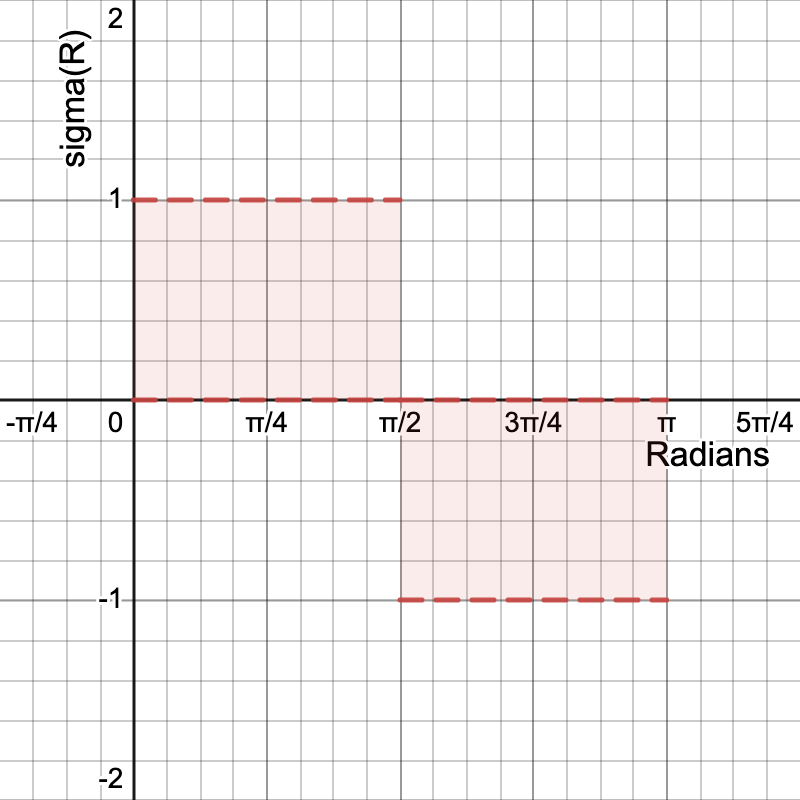
\includegraphics[width=0.42\columnwidth]{sigmaontheta.png}
   \label{fig:sigmaontheta}
 }
\hspace{0.2in}
\subfigure[$\sigma$ vs. $\cos{(\theta)}$] {
   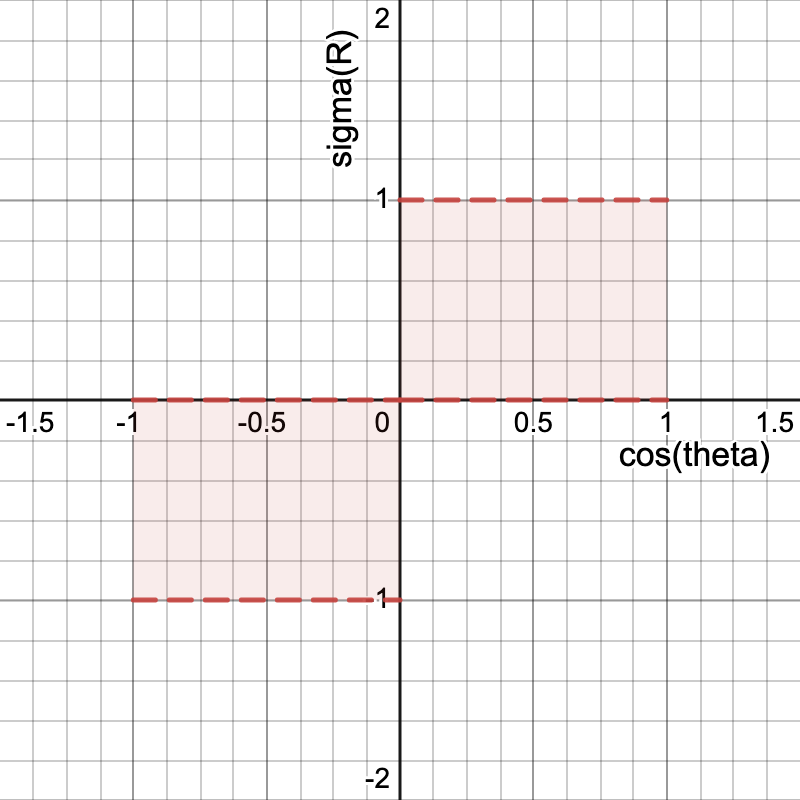
\includegraphics[width=0.42\columnwidth]{sigmaoncos.png}
   \label{fig:sigmaoncos}
 }
\end{center}
\caption{\small Illustration of charge density dependence for problem 3.23.  Left: Dependence of the charge density on $\theta$ at $r=R$  The range of $\theta$ is $0-\pi$.  Right: Dependence of the charge density on $\cos{(\theta)}$.  The range of $\cos{(\theta)}$ is $\pm 1$.}
\label{fig:chargedensity}
\end{figure}

Before applying the orthogonality relation term by term, reduce the work by considering the parity of the last boundary condition.  The $\theta$ dependence of the charge density on the shell ($r=R$) is shown in Fig.~\ref{fig:sigmaontheta}.  The $\cos{(\theta)}$ dependence of the charge density on the shell ($r=R$) is shown in Fig.~\ref{fig:sigmaoncos}.  The dependence of the charge density on $\cos{(\theta)}$ is an odd function over the interval.  If an odd function can be decomposed into constituent functions, none of them will be even functions.  You \textit{cannot} make an odd function with an even component (and vice vs).  The Legendre polynomials are functions of $\cos{(\theta)}$ (or $x$ where $x=\cos{(\theta)}$); those with an even index are even functions, while those with an odd index are odd functions.  (See the Legendre polynomial section of 'Ch3\_L2\_orthogonal\_functions'.)  So, a quick look at parity informs us that $A_{0}$, $A_{2}$, $A_{4}$, $\ldots$ are zero and do not have to be calculated! 

The property of orthogonal functions will be applied to determine the coefficients.  This was given for Legendre polynomial functions in 'Ch3\_L2\_orthogonal\_functions' (Eq. 15 in that lecture) and is restated here:

\begin{equation*}
\int_{-1}^{1} \, P_{l}(x)P_{l^{\prime}}(x) dx = \int_{0}^{\pi} \, P_{l}(\cos{(\theta)})P_{l^{\prime}}(\cos{(\theta)})\sin{(\theta)}d\theta = \frac{2}{2l+1} \delta_{ll^{\prime}}
\end{equation*}

First, the coefficients will be found one-by-one by using orthogonality to selectively solve for each coefficient in turn.  Start by finding $\textcolor{red} {A_{1}}$; to do this multiply Eq.~\ref{eq:hemilast} by the $n=1$ Legendre polynomial (parameterized in terms of $x$ for convenience) $\textcolor{red} {P_{1}(x)}$.  Integration over the interval must be split into two parts since the sign of the charge density changes; that is,  $+\sigma_{0}$ from $x=0$ to $x=1$; and $-\sigma_{0}$ from $x=-1$ to $x=0$.  Remember, all the even terms are zero, so they do not have to be written out.

\begin{eqnarray*}
\frac{1}{\varepsilon_{0}}\left( \int_{0}^{1} \sigma(R,\theta)\textcolor{red} {P_{1}(x)} dx -  \int_{-1}^{0} \sigma(R,\theta) \textcolor{red} {P_{1}(x)} dx \right) & = & 3\textcolor{red} {A_{1}} \int_{-1}^{1} P_{1}(x) \textcolor{red}{P_{1}(x)} dx \\
& + & 7A_{3} R^{2} \int_{-1}^{1} P_{3}(x) \textcolor{red}{P_{1}(x)} dx \\
& + & 11A_{5} R^{4} \int_{-1}^{1} P_{5}(x) \textcolor{red}{P_{1}(x)} dx 
\end{eqnarray*}

This is:

\begin{eqnarray*}
\frac{\sigma_{0}}{\varepsilon_{0}} \left( \int_{0}^{1} \textcolor{red} {P_{1}(x)} dx - \int_{-1}^{0} \textcolor{red} {P_{1}(x)} dx \right) & =  & 3 \textcolor{red} {A_{1}} \left( \frac{2}{2(1)+1} \right) \textcolor{red} {\delta_{11}}\\
& + & 7A_{3}R^{2}   \left( \frac{2}{2(3)+1} \right) \delta_{31}\\
& + & 11A_{5} R^{4} \left( \frac{2}{2(5)+1} \right) \delta_{51}   + \ldots
\end{eqnarray*}

Only the first term on the RHS survives,

\begin{equation*}
\frac{\sigma_{0}}{\varepsilon_{0}} \left( \int_{0}^{1}  x dx - \int_{-1}^{0} x dx \right) =  3\left( \frac{2}{3} \right) A_{1}   + 0 + 0 + \ldots 
\end{equation*}

Solving for $A_{1}$:

\begin{eqnarray*}
\begin{aligned}
 & 2A_{1}  = \frac{\sigma_{0}}{\varepsilon_{0}} \left[ \left. \frac{x^{2}}{2}\right|_{0}^{1} - \left. \frac{x^{2}}{2}\right|_{-1}^{0}\right] = \frac{\sigma_{0}}{\varepsilon_{0}}  \left[ \left( \frac{1}{2} -0 \right) - \left( 0-\frac{1}{2} \right) \right] \\[6pt]
 &  A_{1}  =  \frac{\sigma_{0}}{2\varepsilon_{0}} 
\end{aligned}
\end{eqnarray*}

To find $\textcolor{red} {A_{3}}$, multiply Eq.~\ref{eq:hemilast} by the $n=3$ Legendre polynomial (parameterized in terms of $x$ for convenience) $\textcolor{red} {P_{3}(x)}$ and integrate.

\begin{eqnarray*}
\frac{1}{\varepsilon_{0}}\left( \int_{0}^{1} \sigma(R,\theta)\textcolor{red} {P_{3}(x)} dx -  \int_{-1}^{0} \sigma(R,\theta) \textcolor{red} {P_{3}(x)} dx \right) & = & 3A_{1} \int_{-1}^{1} P_{1}(x) \textcolor{red}{P_{3}(x)} dx \\
& + & 7\textcolor{red} {A_{3}} R^{2} \int_{-1}^{1} P_{3}(x) \textcolor{red}{P_{3}(x)} dx \\
& + & 11A_{5} R^{4} \int_{-1}^{1} P_{5}(x) \textcolor{red}{P_{3}(x)} dx 
\end{eqnarray*}

This is,

\begin{eqnarray*}
\frac{\sigma_{0}}{\varepsilon_{0}} \left( \int_{0}^{1} \textcolor{red} {P_{3}(x)} dx - \int_{-1}^{0} \textcolor{red} {P_{3}(x)} dx \right) & =  & 3 A_{1} \left( \frac{2}{2(1)+1} \right) \delta_{13}\\
& + & 7\textcolor{red} {A_{3}} R^{2}   \left( \frac{2}{2(3)+1} \right) \textcolor{red} {\delta_{33}}\\
& + & 11A_{5} R^{4} \left( \frac{2}{2(5)+1} \right) \delta_{53}   + \ldots
\end{eqnarray*}

Only the 2nd term on the RHS survives,

\begin{eqnarray*}
\frac{\sigma_{0}}{\varepsilon_{0}} \left( \int_{0}^{1}  \frac{1}{2}(5x^{3}-3x) dx - \int_{-1}^{0} \frac{1}{2}(5x^{3}-3x) dx \right) & = &  0 + 7R^{2}\left( \frac{2}{7} \right) A_{3} + 0 + \ldots  \\[4pt]
\frac{\sigma_{0}}{2\varepsilon_{0}}\left[ \left. \left( \frac{5}{4}x^{4}-\frac{3}{2}x^{2} \right) \right|_{0}^{1} -  \left. \left( \frac{5}{4}x^{4}-\frac{3}{2}x^{2} \right) \right|_{-1}^{0} \right] & = &  2R^{2} A_{3}   \\[4pt]
\frac{\sigma_{0}}{2\varepsilon_{0}}\left[ \left( \frac{5}{4}-\frac{3}{2} - 0 \right)  -  \left( 0 - \left( \frac{5}{4}-\frac{3}{2} \right) \right)  \right] & = &  2R^{2} A_{3} 
\end{eqnarray*}

Solving for $A_{3}$:
\begin{equation*}
 A_{3} = \frac{\sigma_{0}}{4R^{2}\varepsilon_{0}}2\left( \frac{5}{4} - \frac{6}{4} \right) = - \frac{\sigma_{0}}{8R^{2}\varepsilon_{0}}
\end{equation*}

To find $\textcolor{red} {A_{5}}$, multiply Eq.~\ref{eq:hemilast} by the $n=5$ Legendre polynomial (parameterized in terms of $x$ for convenience) $\textcolor{red} {P_{5}(x)}$ and integrate.

\begin{eqnarray*}
\frac{1}{\varepsilon_{0}}\left( \int_{0}^{1} \sigma(R,\theta)\textcolor{red} {P_{5}(x)} dx -  \int_{-1}^{0} \sigma(R,\theta) \textcolor{red} {P_{5}(x)} dx \right) & = & 3A_{1} \int_{-1}^{1} P_{1}(x) \textcolor{red}{P_{5}(x)} dx \\
& + & 7 A_{3} R^{2} \int_{-1}^{1} P_{3}(x) \textcolor{red}{P_{5}(x)} dx \\
& + & 11 \textcolor{red} {A_{5}} R^{4} \int_{-1}^{1} P_{5}(x) \textcolor{red}{P_{5}(x)} dx 
\end{eqnarray*}

This is,

\begin{eqnarray*}
\frac{\sigma_{0}}{\varepsilon_{0}} \left( \int_{0}^{1} \textcolor{red} {P_{5}(x)} dx - \int_{-1}^{0} \textcolor{red} {P_{5}(x)} dx \right) & =  & 3 A_{1} \left( \frac{2}{2(1)+1} \right) \delta_{15}\\
& + & 7 A_{3} R^{2}   \left( \frac{2}{2(3)+1} \right) \delta_{35}\\
& + & 11\textcolor{red} {A_{5}} R^{4} \left( \frac{2}{2(5)+1} \right) \textcolor{red} {\delta_{55}}   + \ldots
\end{eqnarray*}

Only the 3rd term on the RHS survives,

\begin{eqnarray*}
\frac{\sigma_{0}}{8\varepsilon_{0}} \left( \int_{0}^{1} (63x^{5}-70x^{3}+15x) dx - \int_{-1}^{0}  (63x^{5}-70x^{3}+15x) dx \right) & = &  11R^{4}\left( \frac{2}{11} \right) A_{5}  \\[4pt]
\frac{\sigma_{0}}{8\varepsilon_{0}}\left[ \left. \left( \frac{63}{6}x^{6}-\frac{70}{4}x^{4}+ \frac{15}{2} x^{2} \right) \right|_{0}^{1} -  \left. \left( \frac{63}{6}x^{6}-\frac{70}{4}x^{4}+\frac{15}{2} x^{2} \right) \right|_{-1}^{0} \right] & = &  2R^{4} A_{5}   \\[4pt]
\frac{\sigma_{0}}{8\varepsilon_{0}}\left[ \left( \frac{126}{12}-\frac{210}{12} + \frac{90}{12} - 0 \right)  -  \left( 0 - \left( \frac{126}{12}-\frac{210}{12} + \frac{90}{12} \right) \right)  \right] & = &  2R^{4} A_{5} 
\end{eqnarray*}

Solving for $A_{5}$:
\begin{equation*}
 A_{5} = \frac{\sigma_{0}}{96R^{4}\varepsilon_{0}}\left( 126 - 210 + 90 \right) = \frac{\sigma_{0}}{16R^{4}\varepsilon_{0}}
\end{equation*}

Now that the coefficients are determined (at least the first few) the series expressions for $V_{\text{in}}$ and $V_{\text{out}}$ are completely determined.  Plugging the coefficients into Eq.~\ref{eq:vinzeros} the potential $V_{\text{in}}$ is as follows:
 
\begin{eqnarray*}
V_{\text{in}}(r,\theta) & = & \sum_{l=0}^{\infty} A_{l}r^{l} P_{l}(\cos{(\theta)}) = A_{1}rP_{1}+A_{3}r^{3}P_{3}+A_{5}r^{5}P_{5}+\ldots \\[6pt]
& = & \frac{\sigma_{0}}{2\varepsilon_{0}} \: r \,P_{1} - \frac{\sigma_{0}}{8\varepsilon_{0} R^{2}} \: r^{3} \, P_{3} + \frac{\sigma_{0}}{16\varepsilon_{0} R^{4}} \: r^{5} \, P_{5}+\ldots  \\[6pt]
\end{eqnarray*}
The above notation with symbols for the Legendre polynomials (such as $P_{1}$) is compact and convenient.  However, for the sake of completeness, $V_{\text{in}}(r,\theta)$ written out in terms of $r$ and $\cos{(\theta)}$ would be:

\begin{align}
&  V_{\text{in}}(r,\theta) = \frac{\sigma_{0}}{2\varepsilon_{0}} \, r \, \cos{(\theta)} - \frac{\sigma_{0}}{8\varepsilon_{0}} \, \left(\frac{r^{3}}{R^{2}}\right) \, \left( \frac{5}{2}\cos^{3}{(\theta)} - \frac{3}{2}\cos{(\theta)} \right) \notag \\[6pt]
& \hspace{.5in} + \frac{\sigma_{0}}{16\varepsilon_{0}} \, \left(\frac{r^{5}}{R^{4}}\right) \, \left( \frac{63}{8}\cos^{5}{(\theta)}-\frac{70}{8}\cos^{3}{(\theta)}+\frac{15}{8}\cos{(\theta)} \right) + \ldots \notag
\end{align}

\vspace{.2in}
Finally, plugging the coefficients into Eq.~\ref{eq:voutzeros}, the potential $V_{\text{out}}$ is as follows:
\begin{eqnarray*}
V_{\text{out}}(r,\theta) &  = & \sum_{l=0}^{\infty} A_{l}R^{2l+1}r^{-(l+1)} P_{l}(\cos{(\theta)}) = A_{1}R^{3}r^{-2}P_{1} + A_{3}R^{7}r^{-4}P_{3} + A_{5}R^{11}r^{-6}P_{5} + \ldots \\[6pt]
& = &  \frac{\sigma_{0}}{2\varepsilon_{0}} R^{3}r^{-2}P_{1} -\frac{\sigma_{0}}{8R^{2}\varepsilon_{0}}R^{7}r^{-4}P_{3} + \frac{\sigma_{0}}{16R^{4}\varepsilon_{0}}R^{11}r^{-6}P_{5} + \ldots \\[6pt]
& = &  \frac{\sigma_{0}}{2\varepsilon_{0}} \left( \frac{R^{3}}{r^{2}} \right) P_{1} - \frac{\sigma_{0}}{8\varepsilon_{0}}\left( \frac{R^{5}}{r^{4}} \right) P_{3} + \frac{\sigma_{0}}{16\varepsilon_{0}}\left( \frac{R^{7}}{r^{6}} \right) P_{5} + \ldots 
\end{eqnarray*}


 {\color{grey} \rule{\linewidth}{0.7mm} }\\
 
 \end{flushleft}
\end{document}
 
%Future - add examples



